\documentclass[11pt, letterpaper]{article}

\usepackage[utf8]{inputenc}
\usepackage[T2A]{fontenc}
\usepackage[english,russian]{babel}
\usepackage{indentfirst}
\usepackage{graphicx}
\graphicspath{ {./images/} }

\title{Документация по проекту Maze}
\author{kwukong, jserra, gtoraq}
\date{Март 2023}

\begin{document}

\maketitle

\pagebreak

\section*{Описание}
«Maze» -  это приложение, которое позволяет генерировать и отрисовывать идеальные лабиринты и пещеры. Реализовано на базе GUI-библиотеки Qt на языке программирования C++ стандарта C++17 в парадигме объектно-ориентированного программирования.

\section{Сборка}
Сборка программы настроена с помощью Makefile с набором целей: all, install, uninstall, clean, dvi, dist, tests.

\begin{itemize}
	\item all - компиляция и установка;
	\item install - установка;
	\item uninstall - выполняется удаление всех установленных файлов;
	\item clean - выполняется удаление тех файлов из текущего каталога, которые были созданы при построении программы;
	\item dvi - выполняется построение DVI-файлов для всей TeXinfo-документации;
	\item dist - выполняется создание tar-файла, содержащего дистрибутивную поставку этой программы;
	\item tests - выполняется тестирование с помощью библиотеки Gtest;
\end{itemize}


\section{Основные возможности программы}
Функции лабиринта:

\begin{itemize}
	\item Область рисования, где можно выбрать начальную и конечную точки пути;
	\item Загрузка готового лабиринта из txt-файла;
	\item Выбрать настройки для построения лабиринта: высота и ширина;
	\item Сохранение сгенерированного лабиринта в txt-файл.
\end{itemize}

Функции пещеры:

\begin{itemize}
	\item Область рисования, где будет запущена симуляция генерации пещеры;
	\item Загрузка готовой пещеры из txt-файла;
	\item Выбрать настройки для построения пещеры: высота, ширина и шанс начальной инициализации клетки;
	\item Задать лимиты «рождения» и «смерти» клетки;
\end{itemize}


\section{Как пользоваться}
При первом запуске, необходимо выбрать реализацию "Лабиринт" или "Пещера".

При выборе Лабиринт:
\begin{itemize}
	\item Нужно либо загрузить лабиринт, либо нажать кнопку "Сгенерировать". 
	\item Вы можете изменить высоту и ширину лабиринта. Максимальный размер лабиринта - 50х50.
	\item Выберите начальную точку левой кнопкой мыши и конечную точку правой кнопкой мыши.
\end{itemize}


 При выборе Пещера:
 \begin{itemize}	
	\item Нужно либо загрузить пещеру, либо нажать кнопку "Сгенерировать". 
	\item Вы можете изменить высоту и ширину пещеры. Максимальный размер пещеры - 50х50.
	\item Выбрать шанс на начальную инициализацию клетки.
	\item Задать лимиты "рождения" и "смерти" клетки. Пределы "рождения" и "смерти" могут иметь значения от 0 до 7.
	\item По нажатию на кнопку "Пошагово" отрисовывается очередная итерация работы алгоритма.
	\item По нажатию на кнопку "Авто" запускается отрисовка итераций работы алгоритма с частотой 1 шаг в N миллисекунд, где число миллисекунд N задаётся Вами.
\end{itemize}


\section{Вид программы}

\begin{itemize}
	\item Рис. 1: Главное окно Лабиринта
	\item Рис. 2: Главное окно Пещеры
\end{itemize}

\begin{figure}[htb]
    \begin{center}
       \leavevmode
       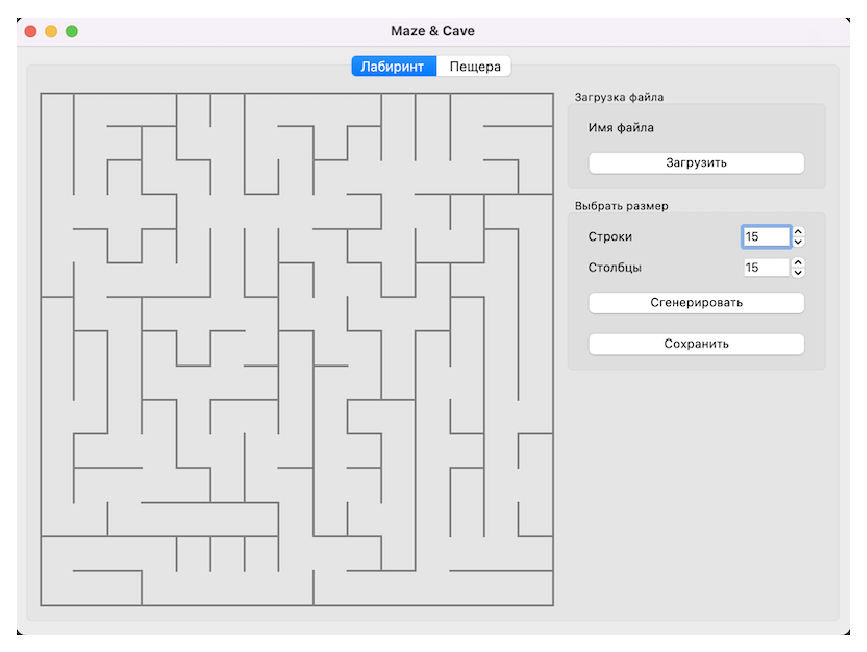
\includegraphics[]{maze.eps}
       \caption{Maze}
    \end{center}
\end{figure}

\begin{figure}[htb]
    \begin{center}
       \leavevmode
       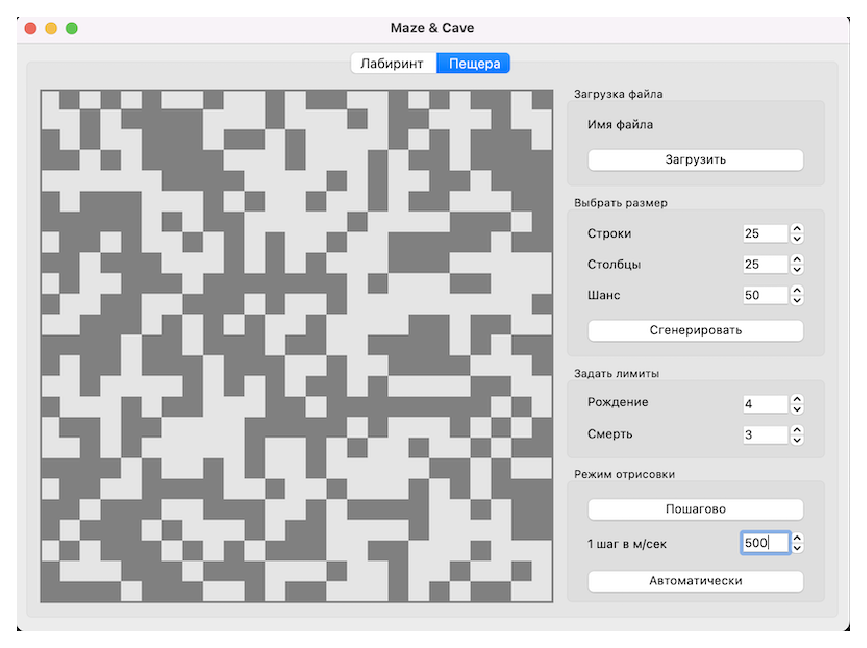
\includegraphics[]{cave.eps}
       \caption{Cave}
    \end{center}
\end{figure}


\end{document}


